% Containment Tree

The CubeSat Reference Architecture is a large model, so the organizational structure is critically important. Many users of this model will be new to MBSE or at least new to Cameo Systems Modeler, and with so many diagrams and packages, it can be easy to get lost or have trouble finding a diagram that you need. Furthermore, modelers may prefer different navigational styles. Some prefer visual diagrams, while others prefer navigating a nested folder structure, while others still may prefer to directly navigate to a desired diagram with one click from an index. To address these preferences, multiple ways to navigate the model have been provided. Each navigation style is based off the four pillars of SysML - Requirements, Structure, Behavior, and Parametrics \citep{SysML}. This model uses the term analysis instead of parametrics to cover more content, but does contain the parametric diagrams to assess system performance. The extra package, called Document Generators, contains templates that pull information from each of other packages, so it is kept separate. 

The standard way is to navigate using the "Containment Tree," or Cameo's File Tree, as shown in Figure \ref{fig:Containment Tree}. Notice the numbered packages for the most important packages to guide users to the appropriate section. Note that some packages, such as those inside the Generic CubeSat Model, include hyperlink icons, informing the user that those packages are also links to more detailed diagrams. A user can navigate this tree and find the appropriate diagrams in an intuitive manner. For example, if they wish to work on the CubeSat's physical decomposition, they will navigate to the Structure package and find the CubeSat package within. If they need to generate some activity diagrams for mission phases, those diagrams will be located within the Behavior section, and so on. 

\begin{figure}[H]
    \centering
    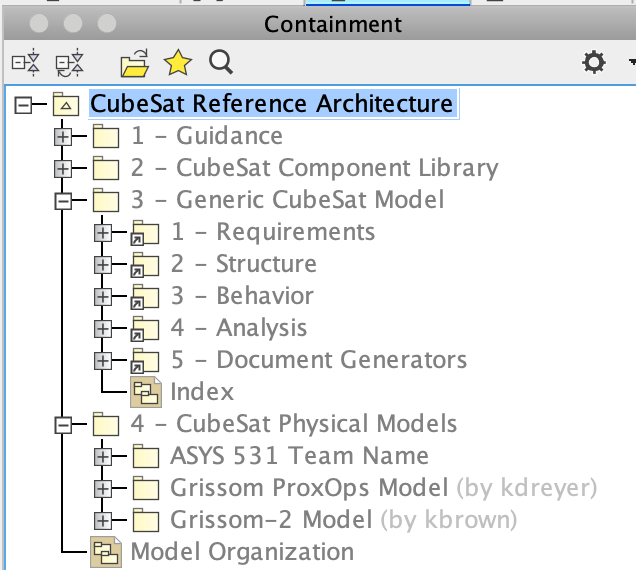
\includegraphics[width=4 in]{Thesis/Analysis_and_Results/Analysis and Results Figures/Containment Tree.png}
    \caption{Containment Tree}
    \label{fig:Containment Tree}
\end{figure}

Some users may prefer to navigate using diagrams instead. This has been built in to the Reference Architecture by creating top level "organization diagrams" for the most used sections. Figure \ref{fig:Model Organization} shows the first page users see when they open up the model, and each icon within that diagram is hyperlinked to another, similar diagram at the lower level. These organization diagrams will be detailed in upcoming sections.

\begin{figure}[H]
    \centering
    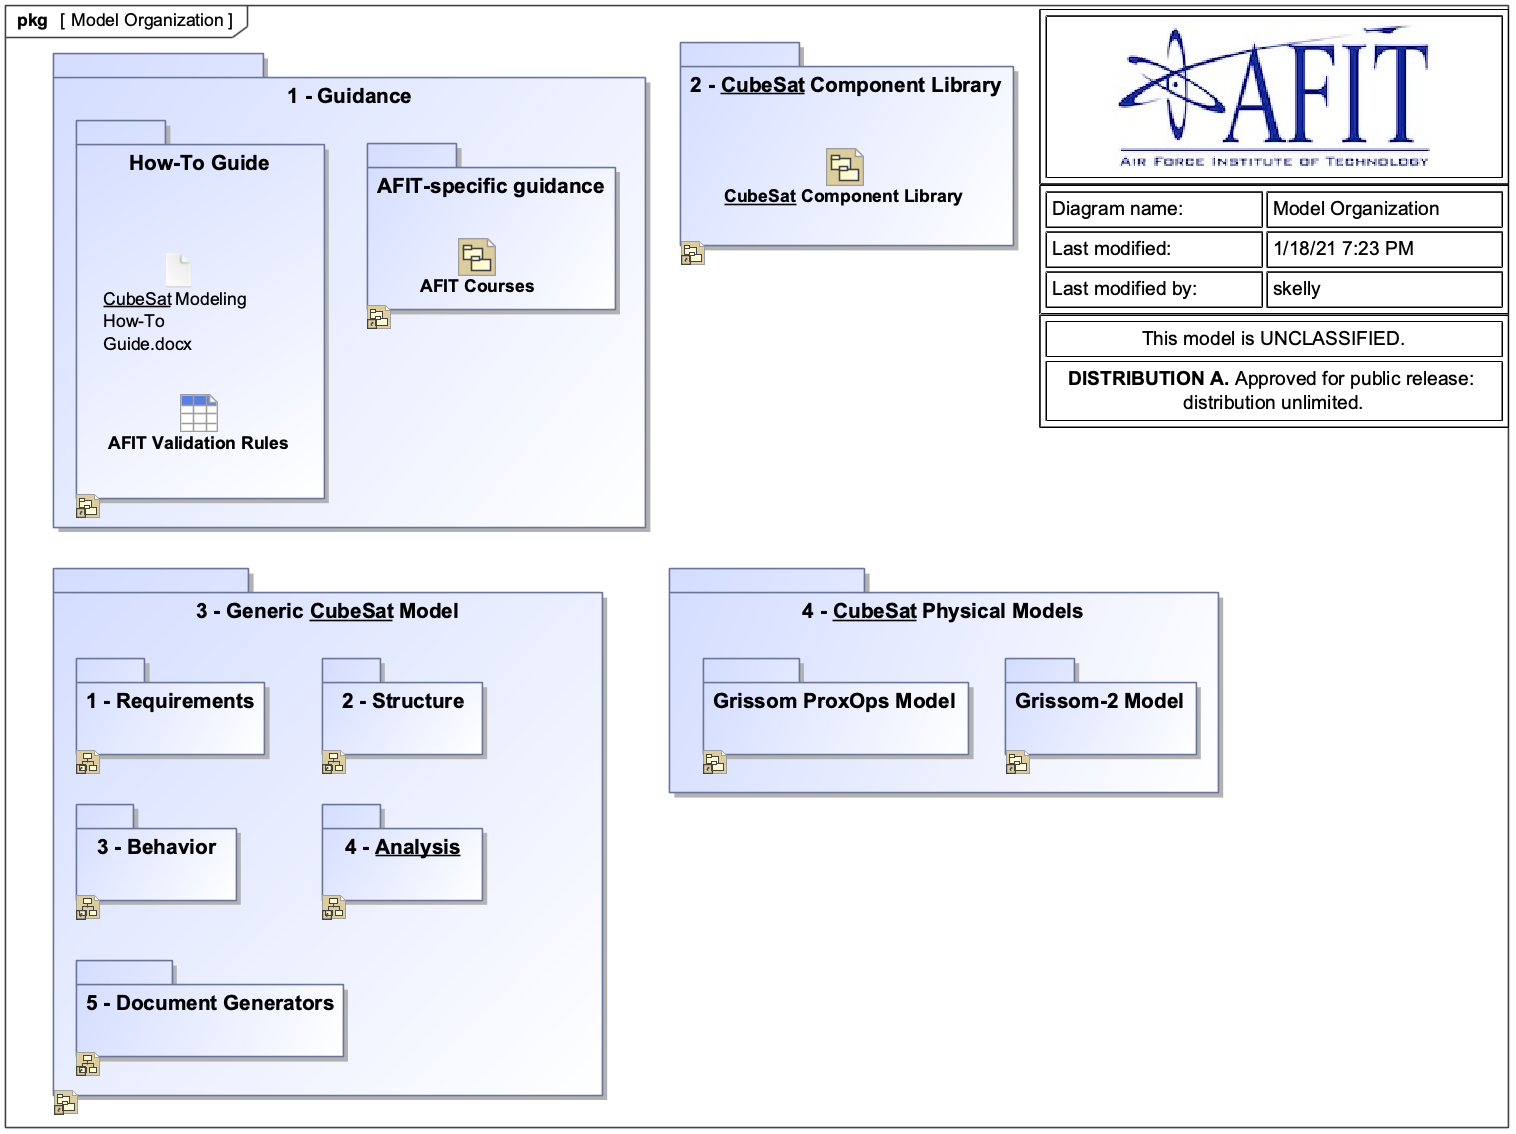
\includegraphics[width=\textwidth]{Thesis/Analysis_and_Results/Analysis and Results Figures/Model Organization.png}
    \caption{Model Organization}
    \label{fig:Model Organization}
\end{figure}

Finally, some users may wish to directly navigate to a diagram by name. The "Index" diagram shown in Figure \ref{fig:Index} shows all of the built-in diagrams and tables that users will be expected to complete during the design sequence, organized by category. If additional diagrams are created, this index will need to be updated accordingly. This Index provides a very fast and easy way to open up one diagram in particular if the user forgot where a diagram was located, for example. 

\begin{figure}[H]
    \centering
    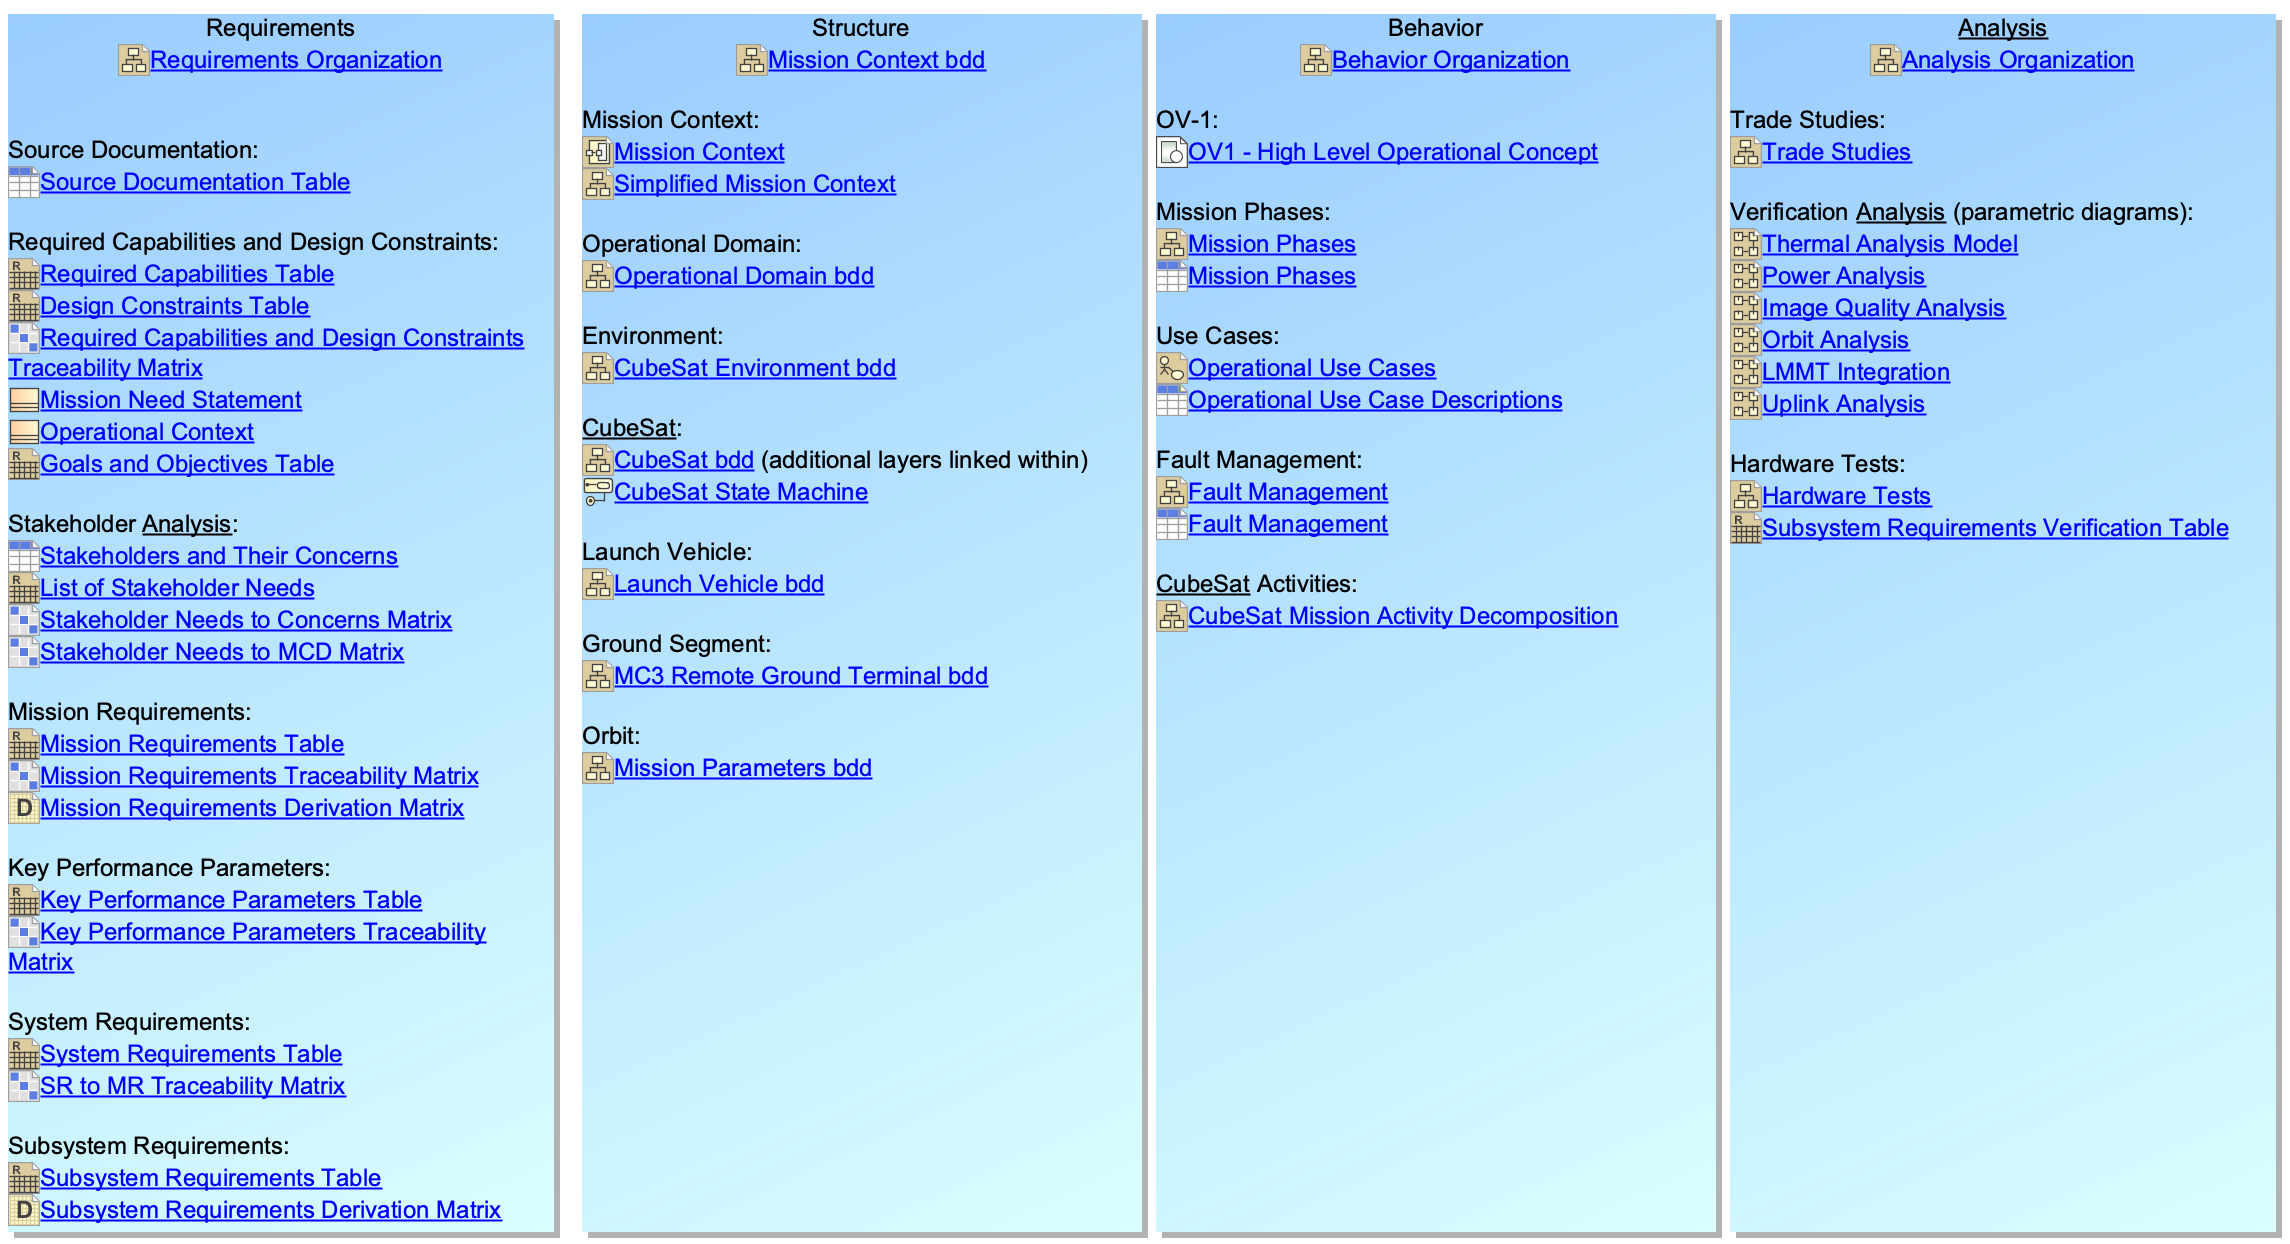
\includegraphics[scale=0.5, angle=90]{Thesis/Analysis_and_Results/Analysis and Results Figures/index.png}
    \caption{Index}
    \label{fig:Index}
\end{figure}